\documentclass[a4paper,10pt]{scrartcl}
\usepackage[utf8]{inputenc}
\usepackage{times}
\usepackage[ngerman]{babel}
\usepackage{amsmath}
\usepackage{amsfonts}
\usepackage{amssymb}
\usepackage{fancyhdr}
\usepackage{graphicx}
\usepackage{listings}
\usepackage{pdfpages} 
\usepackage{listings}
\usepackage[lmargin=2cm,rmargin=2cm,tmargin=2cm,bmargin=2cm]{geometry}

\inputencoding{utf8}
\parindent0em
\pagestyle{fancy}

%opening
\fancyhf{}
%%Titel der Veranstaltung -- Ersetze X durch Zettelnr.
\fancyhead[L]{\textbf{}}
%%Dein Name
\fancyhead[C]{\textbf{}}
%%Dein Tutor
\fancyhead[R]{\textbf{}}
%%\fancyfoot[C]{\thepage}

\newcommand{\M}{\begin{pmatrix}}
\newcommand{\m}{\end{pmatrix}}
\newcommand{\Pt}{\begin{Vmatrix}}
\newcommand{\pt}{\end{Vmatrix}}
           
        
        
\newcommand{\e}{ \mathrm e}
\renewcommand{\i}{ \mathrm i}
\newcommand{\arsinh}{\mathrm{arsinh}}
\newcommand{\rang}{\mathrm{rang}}
\newcommand{\zz}{\mathrm{\hbox{Z}\kern-.4em\raise-0.4ex\hbox{Z}} \hbox{: } }
\newcommand{\mb}[1]{\mathbb{#1}}

\let\stdsubsection\subsection
\renewcommand\subsection{\nopagebreak\stdsubsection}

\begin{document}

\tableofcontents

\section{how to run}

\subsection{Animationenginekonfiguration?}

\subsection{gesturebinding}

\subsection{BML-Aufruf}

\begin{lstlisting}[language=XML]
<bml id="bml1" xmlns="http://www.bml-initiative.org/bml/bml-1.0">
    <postureShift id="pose1" start="0">
        <stance type="STANDING"/>
        <pose part="BODY" lexeme="IDLE"/>
    </postureShift>
</bml>
 \end{lstlisting}

\subsubsection{Parameter}
Klassen? Mocaps?


\section{Description of used techniques with references to literature}

\subsection{MotionGraphs}

The Graph after loading the motion-data. The indices are indices like in our implementation.

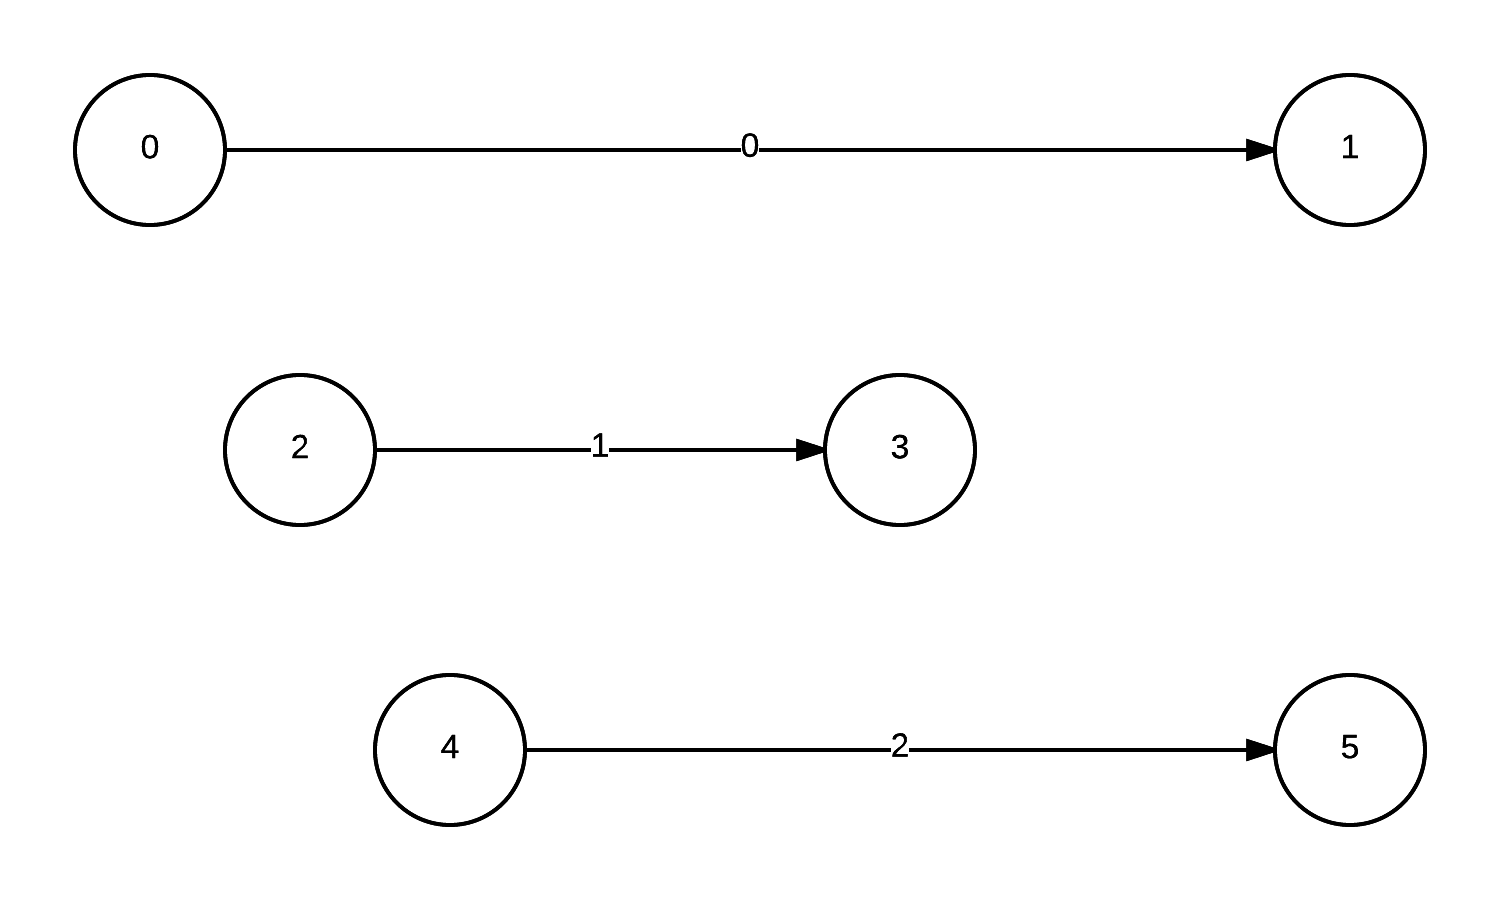
\includegraphics[width=\textwidth/2]{img/1_GraphAtStart.png}


After loading the graph we split motions. Currently, we split motions in equally long pieces.
After splitting, the graph looks as follows.

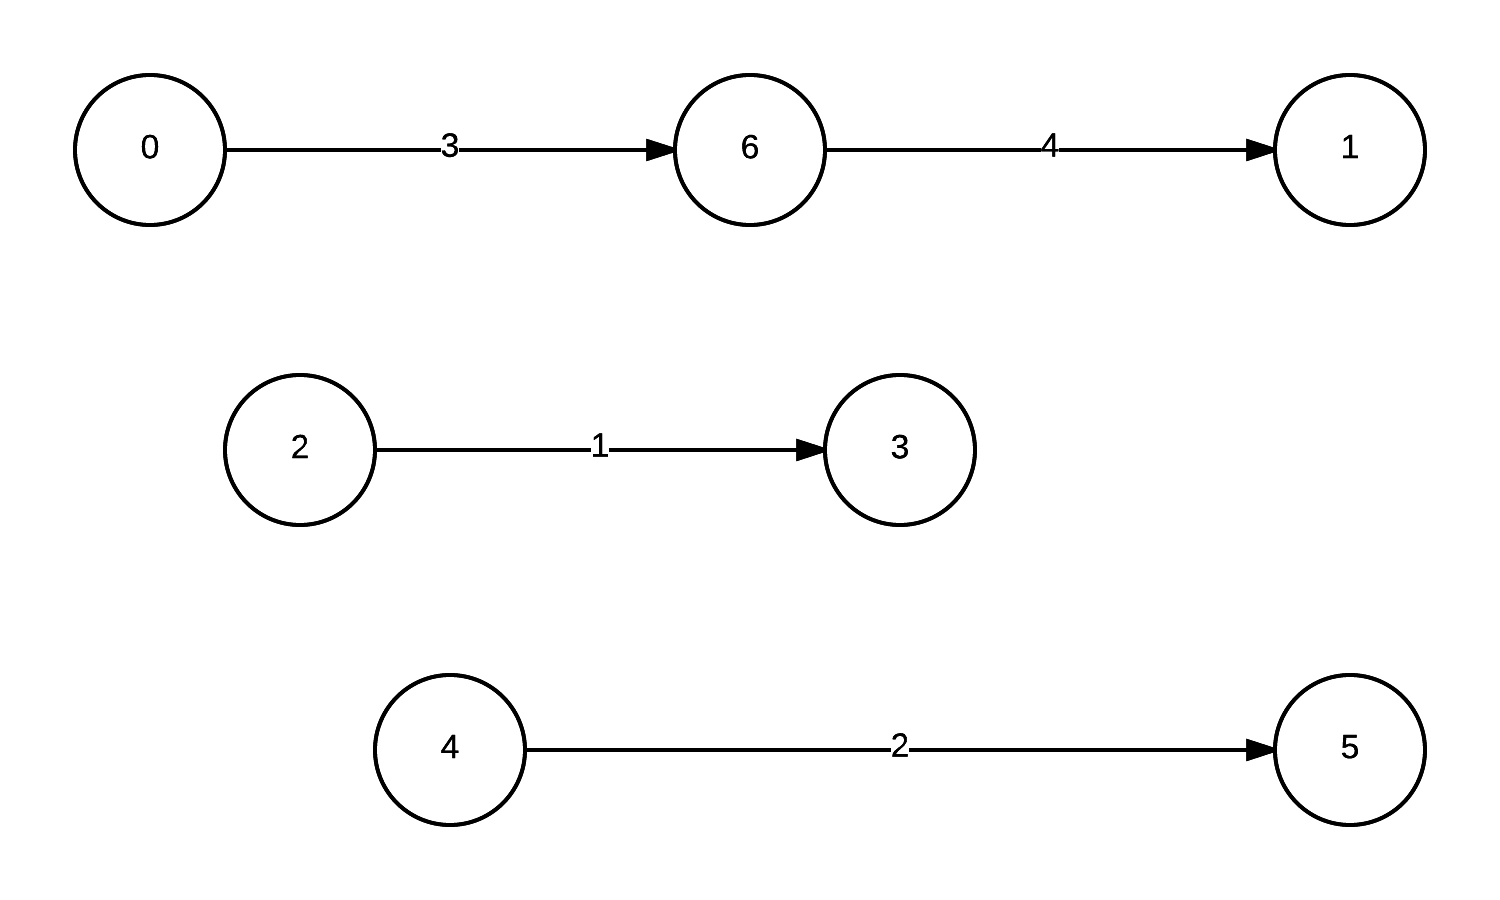
\includegraphics[width=\textwidth/2]{img/2_GraphAfterSplit.png}


After splitting, we use a DistanceMetric to found motions, which are equally enough for Blending.
\\
To blend to motions, we cut both in half, where the end-piece of the first and the start-piece of the second motion are the parts used for blending and so the same length. The blended motion then connects the start-piece of first and the end-piece of the second motion.
\\
In the example, motion 3 should be blended with motion 1, so both are cut in half, 3 in 5 and 6, 1 in 7 and 8. Then, motion 6 and motion 7 are blended to create motion 9, wich now connects motion 5 and 8.
\\
The connected motions 5,9 and 8 are now a smooth transition from node 0 to 3.
 
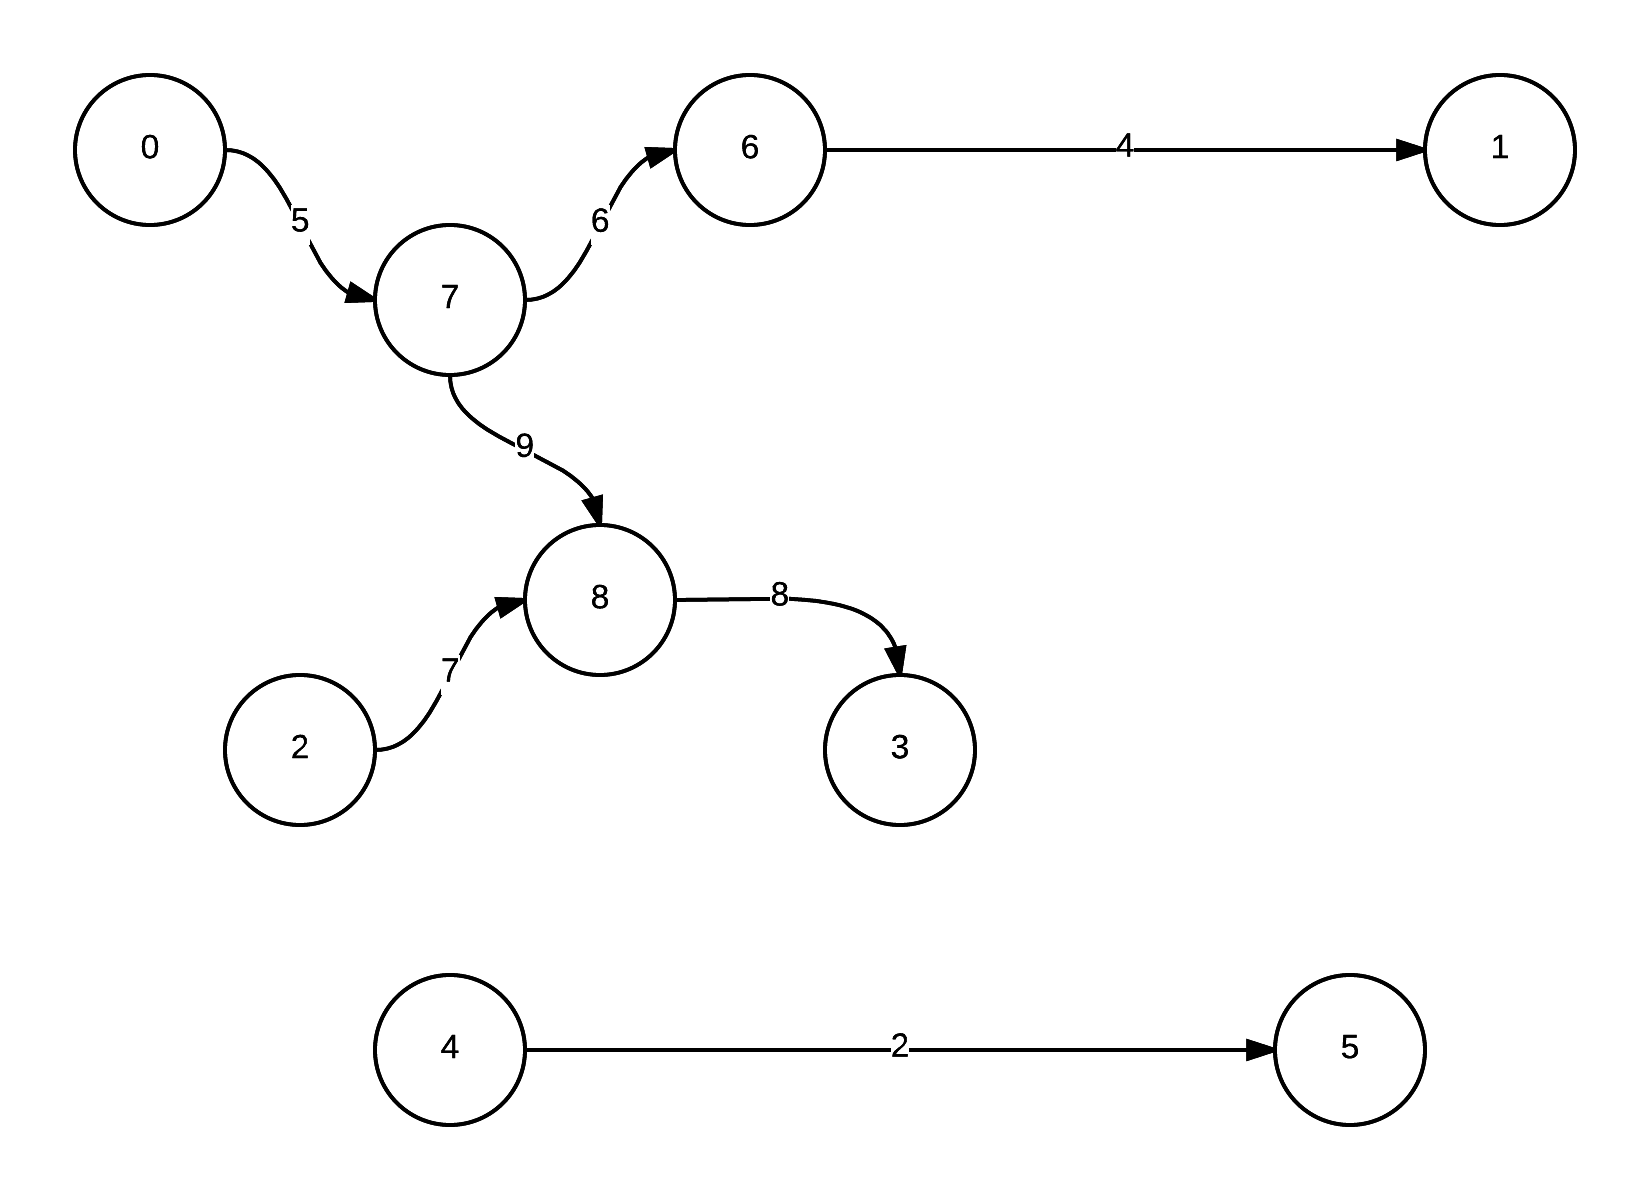
\includegraphics[width=\textwidth/2]{img/3_GraphAfterBlend_0+1.png}


When all possible Blendings are created, the Graph looks as follows.
\\
It contains already inifinte-length motions, which are concatenations of singe motions, but also Dead-Ends, nodes which have no successor.
If one of these are reached in a random-walk, the random-walk stops, so each of them needs to be removed from the graph.
 
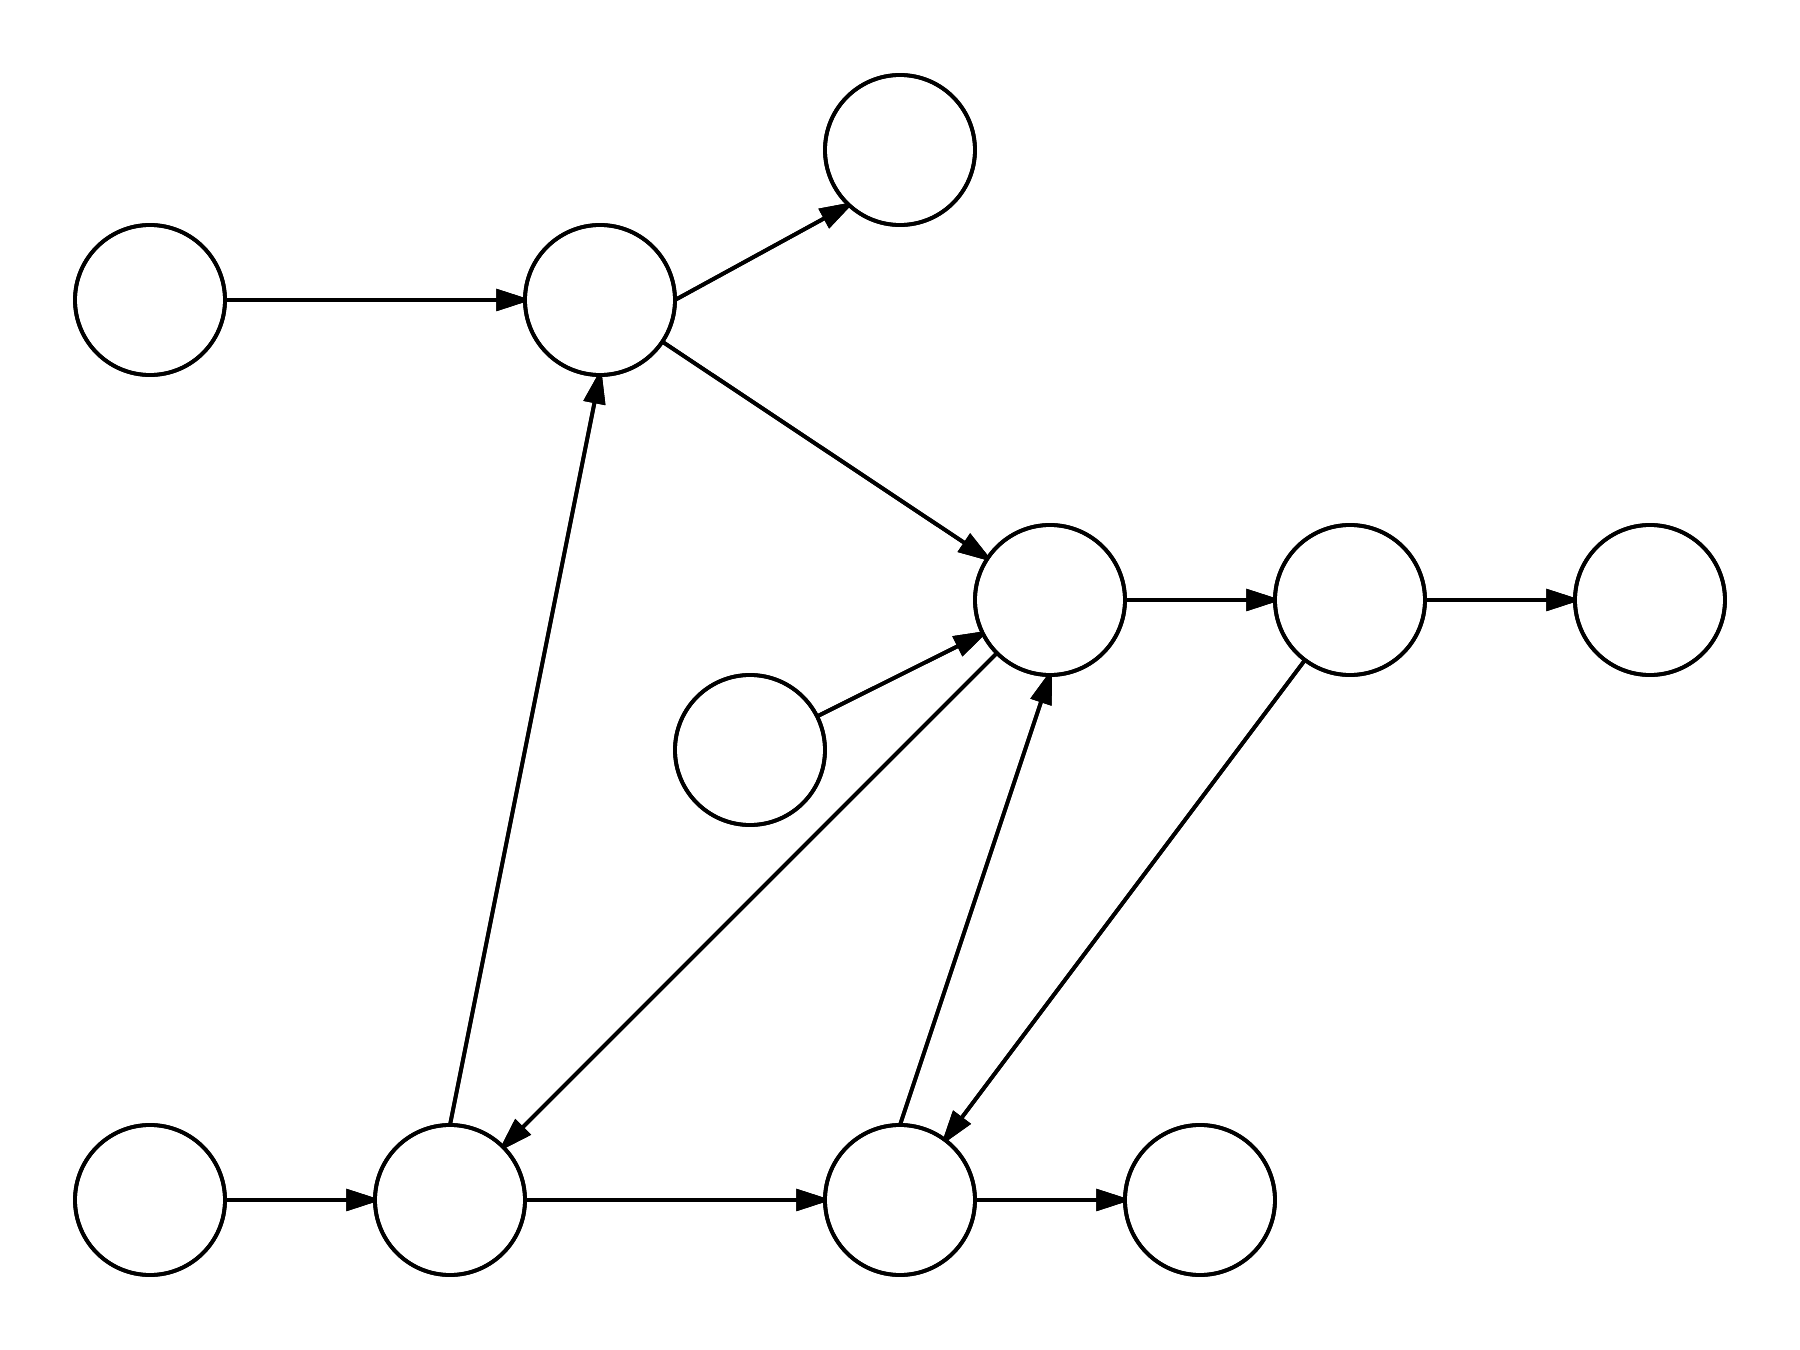
\includegraphics[width=\textwidth/2]{img/4_GraphAfterAllBlends.png}


After pruning, the Graph looks as follows.
\\
Since all Dead-Ends are removed, a random walk could run forever and there's allways a next-motion.

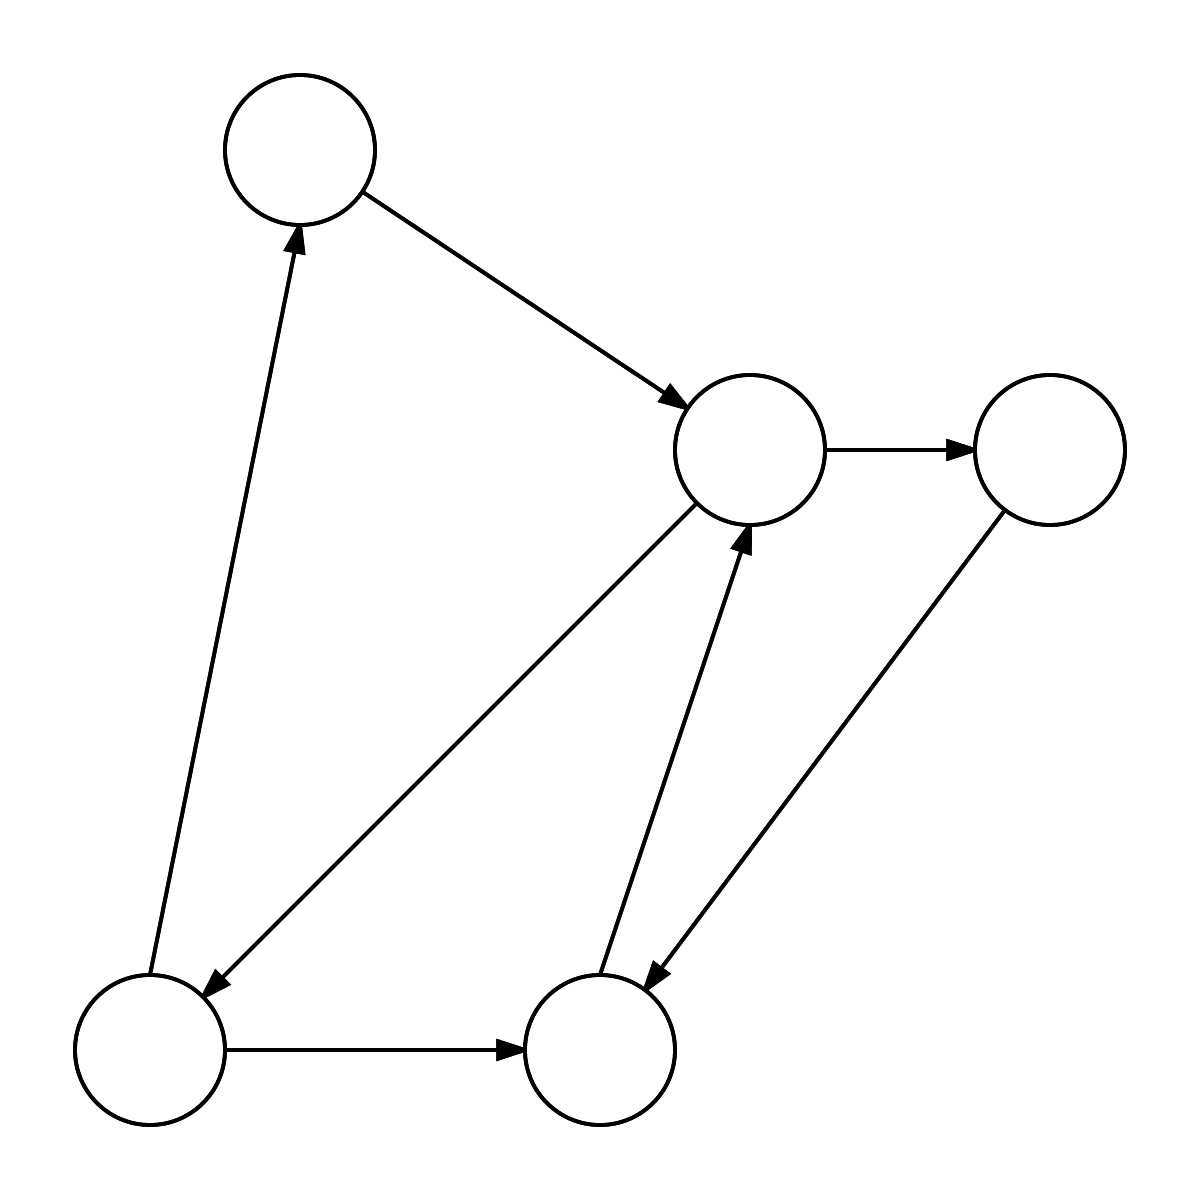
\includegraphics[width=\textwidth/2]{img/5_GraphAfterPruning.png}


\subsection{Distance Metrics}
\subsection{Blending}
\subsection{Align, Split, etc}

\section{System overview (e.g class structure / functional overview / dataflow)}

\subsection{Class structure}
\subsubsection{AbstractMotionGraph}

Interface for MotionGraphs.
Its only Method ist \lstinline[]{next()}, which returns the next Motion in the MotionGraph.

\subsubsection{MotionGraph}

\subsubsection{MotionGraphBuilder}

Our Builder for the MotionGraph. It's implemented to easily construct a MotionGraph with different iplementations for each aspect.
\\
It's not necessary, but was usefull for changing different Parts of the MotionGraph.

\subsubsection{IDistance}

Interface for DistanceMetrics.

\subsubsection{JointAngles}

Our implementation of an DistanceMetric. It's based on the Joint-Angle-Method as described in [vanbasten2009] with few changed.
We only compare root-position and joint angles, and ignore the velocities. Thats mainly beause joint velocities are very low in idle motions and if they are also low-weighted, the tend to be near 0.
\\\\
The weights we use are stored in WeightMap, which holds weights for each joint, ignoring Left/Right.
\\\\
Right now, the weights for arms are very low, and the weights for legs are high.\\
The legs are high, because if they are in different Positions while blend, the slide above the floor. Same doesn't count for arms, since blending of different Positions only leds to new Motions.

\subsubsection{IBlend}

Interface for Blendings

\subsubsection{Blend}
\subsubsection{IAlignment}

Interface for Alignment.

\subsubsection{Alignment}

\subsubsection{ISplit}

Interface for Splitting.
\\\\
We think, a good implementation could split long motions, which contains different, unrelated motions, in piece, which only contains one motion.

\subsubsection{DefaultSplit}

Our Implementation currently splits Motions in pieces with lenght around 2.5 seconds.

\subsubsection{IdleMovement}

The RestPose, which could be started with BML.

It uses the MotionGraph to generate real-looking, infinite Motions for idle-behavior.

\subsection{Startup}
Builder/MotionGraph.init()

\subsection{play()}

\section{Extensibility (e.g. How to use with other mocap files / visemes)}

\subsection{Load mocap}

\subsection{Other Classes?}

%\includepdf[pages={-}]{ueb12.pdf}
\end{document}